\documentclass[pdflatex,compress,mathserif]{beamer}

%\usetheme[dark,framenumber,totalframenumber]{ElektroITK}
\usetheme[darktitle,framenumber,totalframenumber]{ElektroITK}

\usepackage[utf8]{inputenc}
\usepackage[T1]{fontenc}
\usepackage{lmodern}
\usepackage[bahasai]{babel}
\usepackage{amsmath}
\usepackage{amsfonts}
\usepackage{amssymb}
\usepackage{graphicx}
\usepackage{multicol}

\newcommand*{\Scale}[2][4]{\scalebox{#1}{$#2$}}%

\title{PEMODELAN JARINGAN KOMUNIKASI}
\subtitle{Inter-VLAN Routing}

\author{Tim Dosen Pengampu}

\begin{document}
	
\maketitle

\section{Option 1 - Router with Separate Interfaces}

\begin{frame}
	\frametitle{VLANs and IP subnets in the LAN}
	\begin{itemize}
		\item There is typically a one-to-one relationship between an IP subnet and
a VLAN in the LAN campus
		\item For example Engineering hosts are in IP subnet 10.10.10.0/24 and
VLAN 10, and Sales hosts are in IP subnet 10.10.20.0/24 and VLAN 20
		\item Hosts are segregated at Layer 3 by being in different IP subnets, and at
Layer 2 by being in different VLANs
		\item Hosts in different IP subnets need to send traffic via a router to
communicate with each other
	\end{itemize}
\end{frame}

\begin{frame}
	\frametitle{Option 1: Router with separate\\ interfaces}
	\begin{center}
		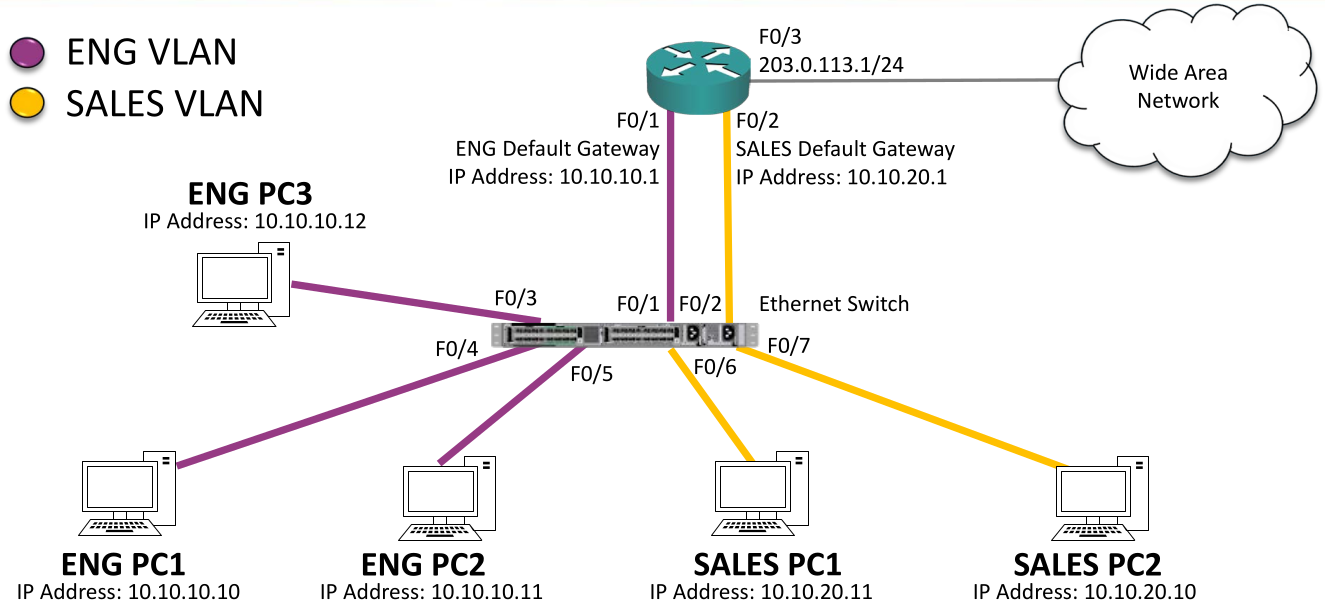
\includegraphics[width=\linewidth]{img/img01}
	\end{center}
\end{frame}

\begin{frame}
	\frametitle{Option 1 Configuration}
	\begin{center}
		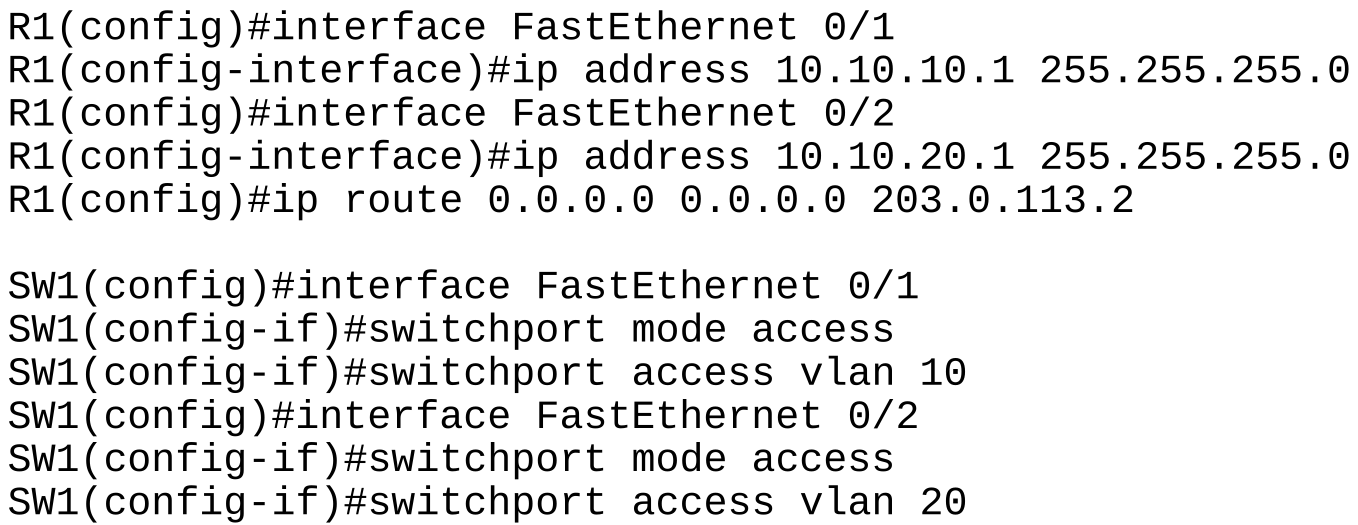
\includegraphics[width=\linewidth]{img/img02}
	\end{center}
\end{frame}

\begin{frame}
	\frametitle{Router with separate interfaces -\\ Disadvantages}
	\begin{itemize}
		\item You need a separate physical interface for every VLAN – you are liable
to run out of interfaces
		\item Traffic being routed within the campus has to go up and down physical
Ethernet cables to the router
	\end{itemize}
\end{frame}

\begin{frame}
	\frametitle{Inter-VLAN Routing Lab}
	\begin{center}
		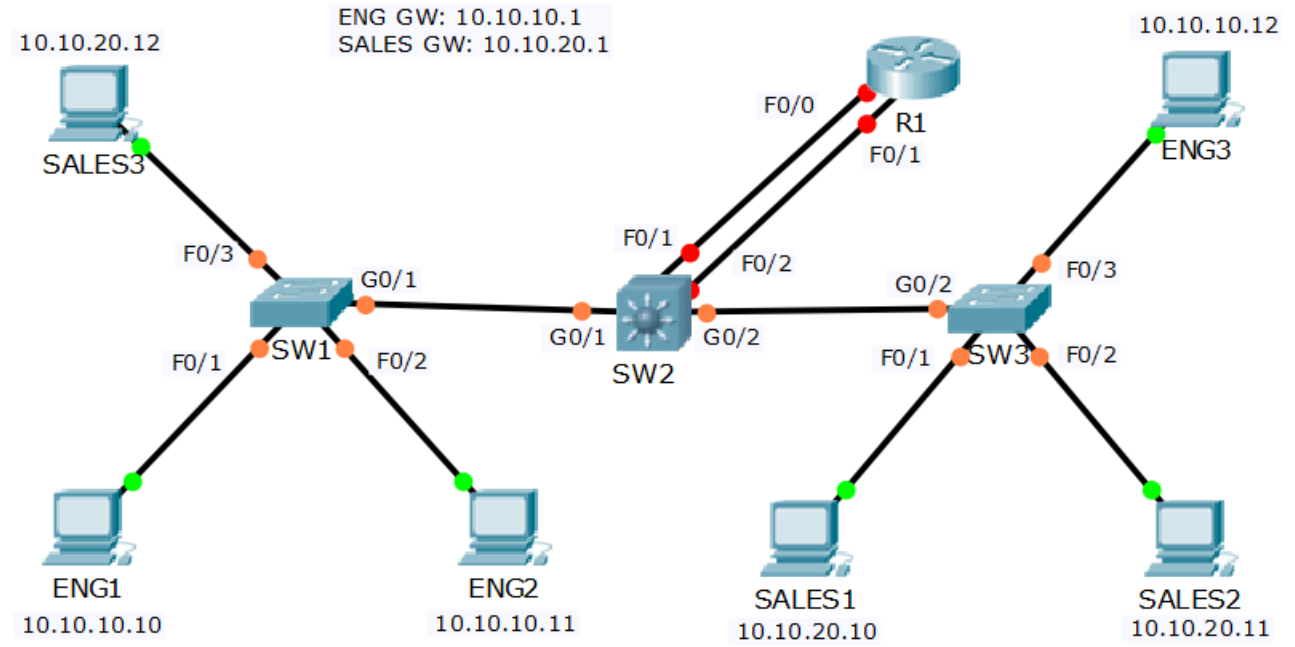
\includegraphics[width=\linewidth]{img/img03}
	\end{center}
\end{frame}

\section{Option 2 - Router on a Stick}

\begin{frame}
	\frametitle{Option 2: Router on a Stick}
	\begin{center}
		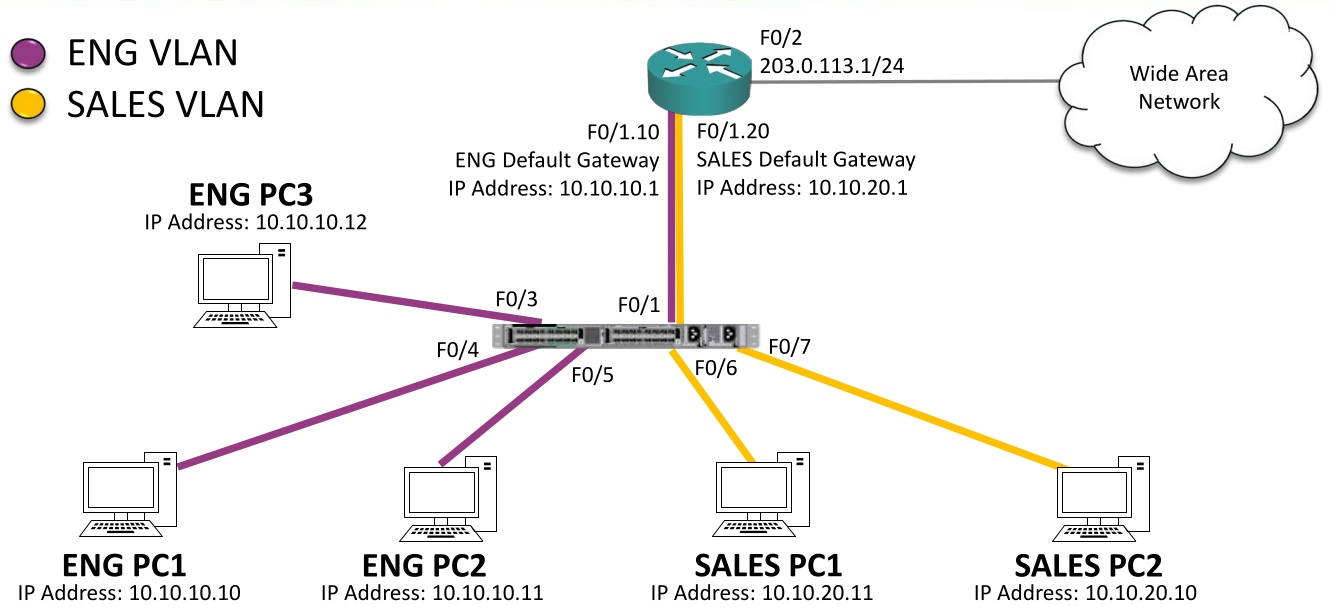
\includegraphics[width=\linewidth]{img/img04}
	\end{center}
\end{frame}

\begin{frame}
	\frametitle{Option 2 Configuration}
	\begin{center}
		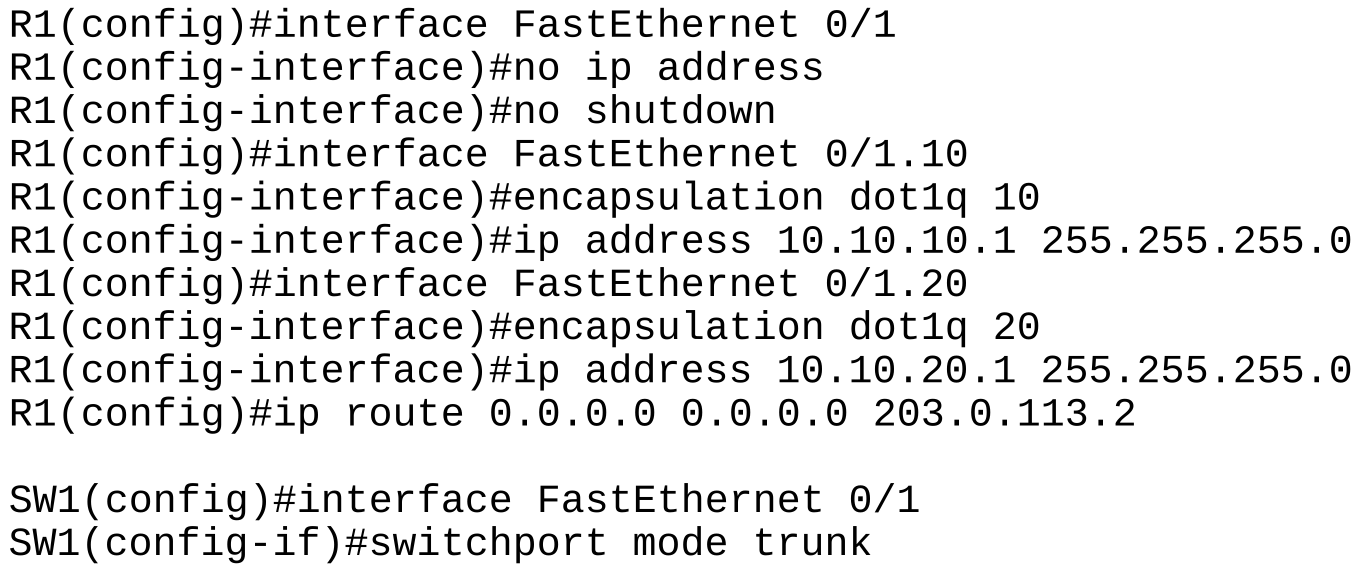
\includegraphics[width=\linewidth]{img/img05}
	\end{center}
\end{frame}

\begin{frame}
	\frametitle{Router on a Stick Considerations}
	\begin{itemize}
		\item You do not need a separate physical interface for every VLAN – you are
less likely to run out of interfaces
		\item Traffic being routed within the campus has to go up and down the
same physical Ethernet cable to the router – there is more contention
for bandwidth than when using separate interfaces
	\end{itemize}
\end{frame}

\begin{frame}
	\frametitle{Inter-VLAN Routing Lab}
	\begin{center}
		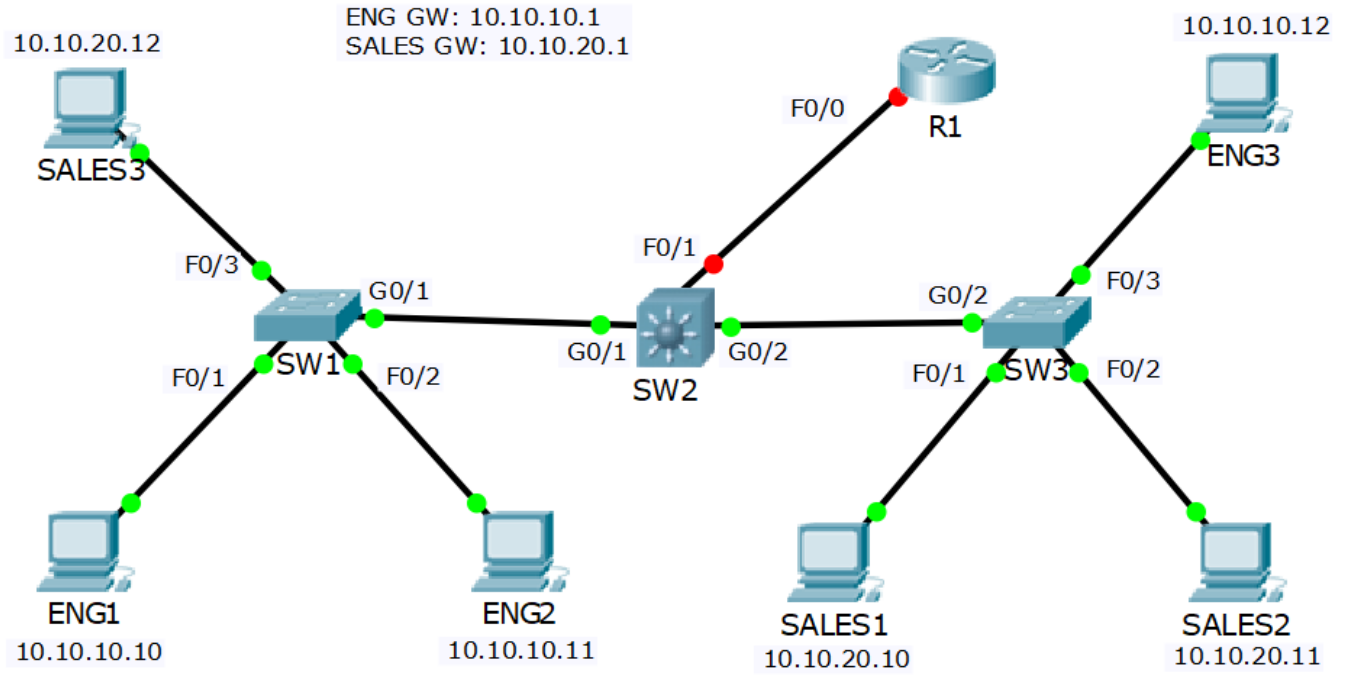
\includegraphics[width=\linewidth]{img/img06}
	\end{center}
\end{frame}

\section{Option 3 - Layer 3 Switch}

\begin{frame}
	\frametitle{Option 3: Layer 3 Switch}
	\begin{center}
		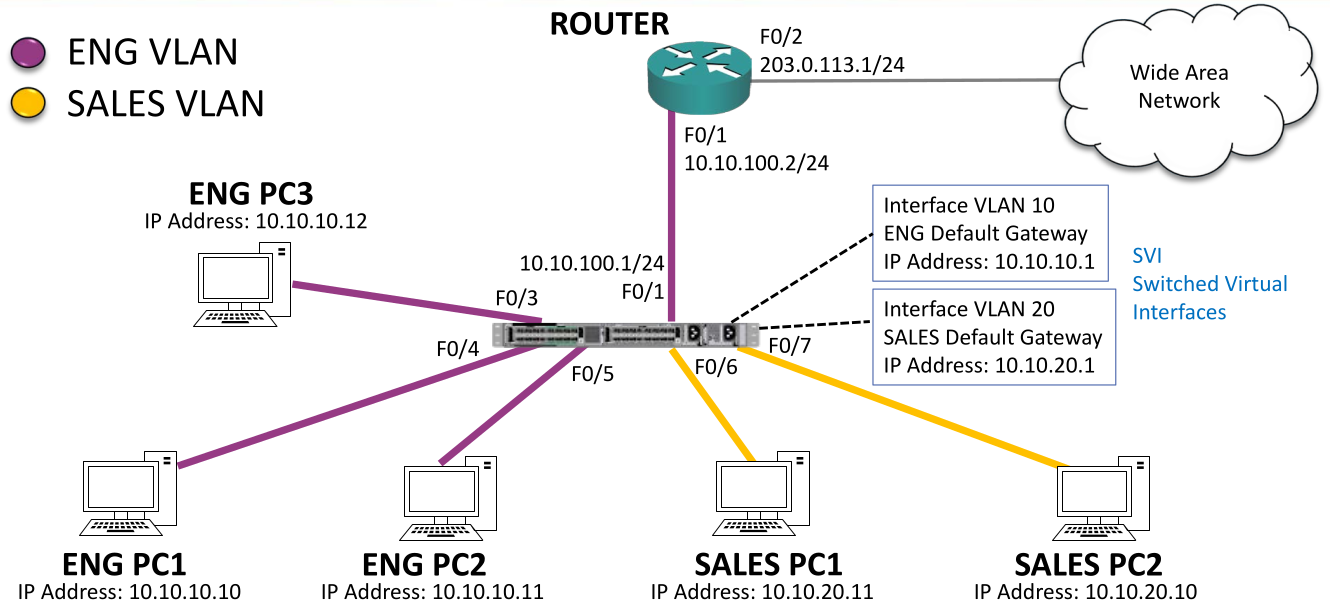
\includegraphics[width=\linewidth]{img/img07}
	\end{center}
\end{frame}

\begin{frame}
	\frametitle{Option 3 Inter-VLAN Routing Configuration}
	\begin{center}
		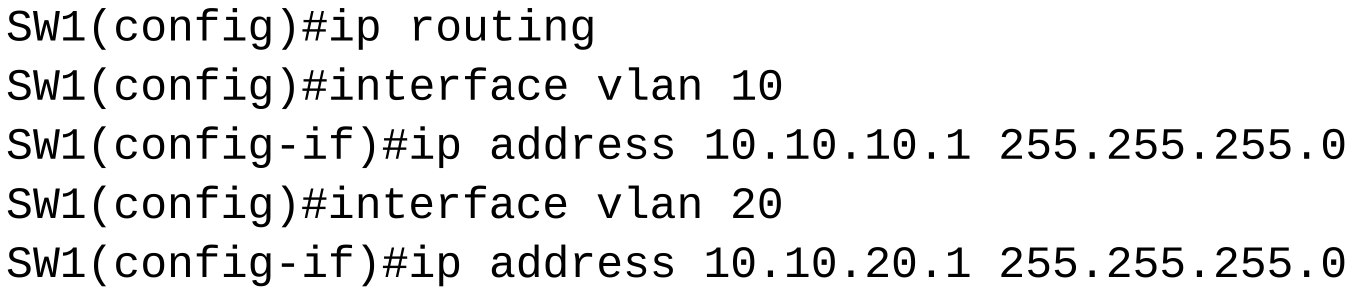
\includegraphics[width=\linewidth]{img/img08}
	\end{center}
\end{frame}

\begin{frame}
	\frametitle{Option 3 WAN Routing Configuration}
	\begin{center}
		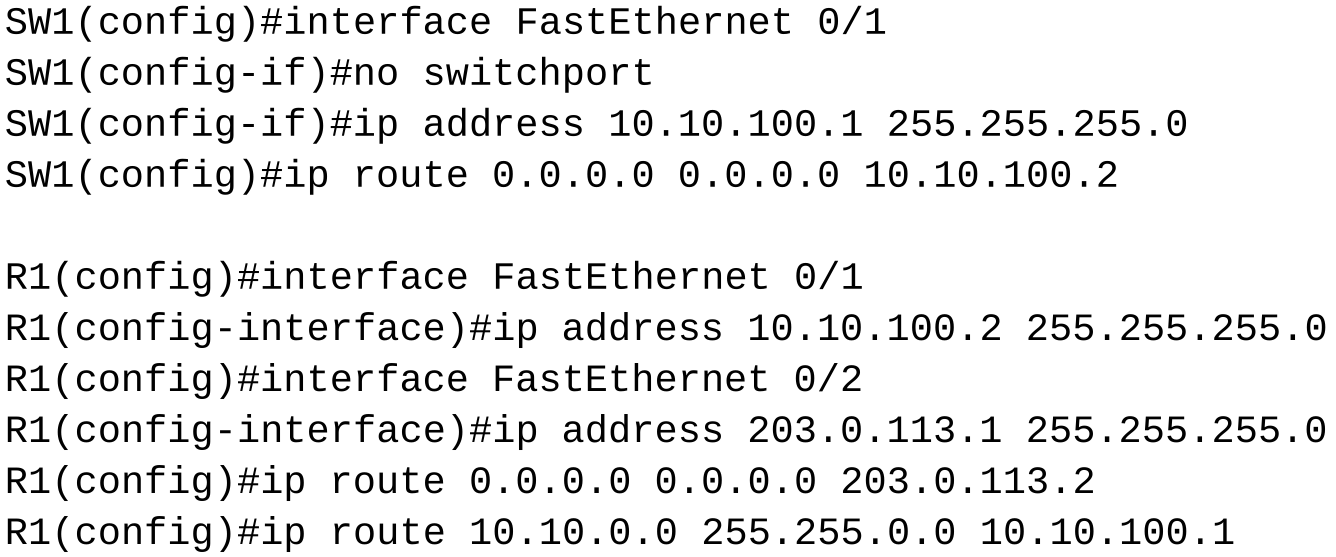
\includegraphics[width=\linewidth]{img/img09}
	\end{center}
\end{frame}

\begin{frame}
	\frametitle{Layer 3 Switch Considerations}
	\begin{itemize}
		\item Traffic being routed within the campus is routed across the switch
backplane, it does not need to travel over physical cables to an
external router
		\item You may still need an external router for WAN connectivity and
services
	\end{itemize}
\end{frame}

\begin{frame}
	\frametitle{Layer 3 Switch Lab}
	\begin{center}
		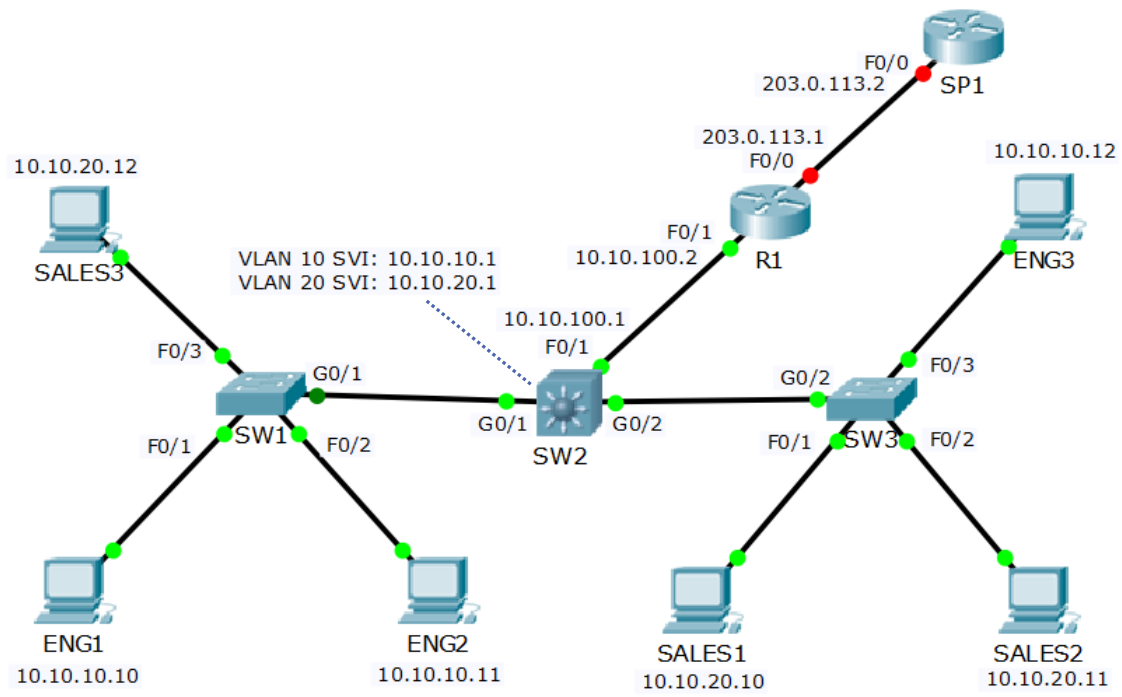
\includegraphics[width=0.9\linewidth]{img/img10}
	\end{center}
\end{frame}

\end{document}